\section{Otras coloraciones}

No todos los problemas se resuelven colorando como tablero de ajedrez. Veamos unos ejemplos.

\begin{ejem}
	Decidir si es posible cubrir completamente un tablero de $10 \times 10 $ con tetramin\'os iguales al de la figura siguiente
	\begin{figure}[h!]
		\centering
		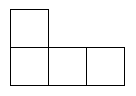
\includegraphics[scale=.8]{imgs/color4.png}
	\end{figure}
\end{ejem}

\begin{proof}
	Empecemos observando que la coloraci\'on de ajedrez no ayuda mucho. Cada ficha subre exactamente dos casillas blancas y dos casillas negras, y hay $50$ casillas blancas y $50$ casillas negras.
	
	Es importante notar que si una coloraci\'on no sirve, ¡Eso no implica que no haya otra coloraci\'on que si sirva!. Apliquemos entonces una vez mas nuestra receta:
	
	\begin{enumerate}[a.]
		
		\item \textit{Colore\'a el tablero}
		
		Para este problema, vamos a colorear las columnas de del tablero de blanco y negro, de manera alternada.
		
		\item \textit{Encontrar una propiedad en la coloraci\'on.}
		
		Podemos observar que, no importa donde se coloque la pieza, siempre estar\'a sobre tres casillas del mismo color y una casilla del color diferente. Es decir, cualquier pieza que se coloque sobre el tablero ocupar\'a una cantidad impar de casillas blancas. Adem\'as, $50$ de las $100$ casillas del tablero son blancas.
		
		\item \textit{Supongamos que la hip\'otesis es falsa}
		
		Es decir, es posible cubrir el tablero completamente, para lo cual necesitaremos $\frac{100}{4} = 25$ piezas. La observaci\'on clave es combinar los dos \'ultimos datos. Estas $25$ piezas cubrir\'an indefectiblemente una cantidad impar (suma de una cantidad impar de n\'umeros impares) de casillas blancas, pero hay $50$ casillas blancas, el cual es un n\'umero par. Luego, es imposible cubrir el tablero.
	\end{enumerate}
\end{proof}

El ojo experto seguro habr\'a notado que \'esta soluci\'on se parece mucho a la del ejemplo \ref{primerejemplo}. No es coincidencia: La virtud de un buen matem\'atico es el saber adaptar soluciones ya vistas a los nuevos desaf\'ios que se le presentan.

\begin{ejem}
	A un tablero de $8 \times 8$ se le ha recortado una casilla de una de las esquinas. Decidir si es posible cubrirlo completamente con fichas de tamaño $3 \times 1$.
\end{ejem}

\begin{proof}
	
	Ya no es ning\'un secreto a la altura de este folleto, vamos a usar la receta:
	
	
	\begin{enumerate}[a.]
		
		\item \textit{Colore\'a el tablero}
		
		Observemos la siguiente coloraci\'on:
		
		\begin{figure}[h!]
			\centering
			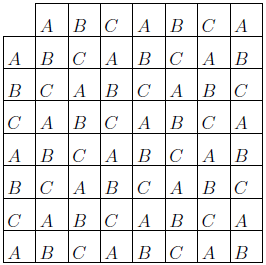
\includegraphics[scale=.85]{imgs/color5.png}
		\end{figure}
		
		\item \textit{Encontrar una propiedad en la coloraci\'on.}
		
		El encanto de \'esta coloraci\'on no es otro sino el siguiente: Cada ficha cubre exactamente una casilla de cada color. 
		
		\item \textit{Supongamos que la hip\'otesis es falsa}
		
		Si el tablero pudiese cubrirse con fichas de $3 \times 1$, entonces deber\'a haber la misma cantidad de casillas de cada color. Eso no ocurre; luego no es posible cubrir el tablero. 
	\end{enumerate}
\end{proof}


Desde luego, las coloraciones que hemos visto no resolver\'an todos los problemas, siempre debemos dejar fluir nuestra imaginaci\'on.

\subsection{Problemas}

\begin{enumerate}
	\item Tenemos un tablero de $7 \times 7$ del cual le hemos recortado una esquina. ¿Es posible cubrirlo con 12 domin\'os verticales y 12 domin\'os horizontales?
	
	\item ¿Cu\'al es la mayor cantidad de casillas que se pueden colorear en un tablero de $7 \times 7 $ de manera que cada subtablero de $2 \times 2$ tiene a lo m\'aximo dos casillas pintadas?
	
	\item Decidir si es posible cubrir completamente un tablero de $10 \times 10$, sin huecos ni superposiciones y sin salirse del tablero, con fichas rectangulares de $1 \times 4$. (Cada ficha debe cubrir exactamente cuatro casillas del tablero.)
	
	\item En cada casilla de un tablero de $12 \times 12$ est\'a escrito un $1$ o un $0$. Una operaci\'on permitida es elegir $5$ casillas consecutivas en direcci\'on vertical, horizontal o diagonal, y con esas $5$ casillas cambiar cada $0$ por $1$ y cada $1$ por $0$. Inicialmente todas las casillas tienen un $0$ escrito en ellas. Determinar si es posible, mediante una secuencia de operaciones permitidas, lograr que todas las casillas del tablero tengan un $1$.
	
	\item Tengo un cuarto cuyo piso tiene forma rectangular y est\'a totalmente cubierto por piezas de azulejos de tamaño $2 \times 2$ y $1\times 4$. Una de las piezas de tamaño $1\times 4$ se ha roto, y solo me queda una pieza de tamaño $2\times 2$ en el dep\'osito. Decidir si es posible reorganizar las piezas que tengo para cubrir completamente mi cuarto de azulejos.
	
	\item Un tablero de $7 \times 7$ se ha cubierto con la m\'axima cantidad posible de fichas de tamaño $3\times 1$. Sin embargo, siempre sobra una casilla. Determine la cantidad de lugares donde esta casilla sobrante puede ubicarse en el tablero.
	
	\item Se tiene un tri\'angulo equil\'atero de lado 7, que est\'a dividido en 49 tri\'angulitos iguales mediante rectas paralelas a sus lados. Se van recortando paralelogramos de per\'imetro 6 formado por cuatro tri\'angulitos de la grilla. Determine la mayor cantidad de paralelogramos que se pueden recortar.
	
	\item Ana y Beto juegan en un tablero de $11$ filas y $9$ columnas. Primero Ana divide el tablero en $33$ zonas. Cada zona tiene la forma de una casilla de tamaño $3\times 1$. 
	
	Luego, Beto escribe en cada casilla uno de los n\'umeros $0, 1, 2, 3, 4, 5$ de modo que la suma de los n\'umeros de cada zona sea igual a 5. Beto gana si la suma de los n\'umeros escritos en cada una de las 9 columnas del tablero es un n\'umero primo. En caso contrario, Ana gana. Demuestre que Beto tiene estrategia ganadora. 
	
	\item Se tiene un tablero de $10\times 4$, en el cual se tiene un caballo en la esquina inferior izquierda. Muestre que no es posible que el caballo realice un ciclo sobre el tablero. Es decir, no puede hacer un recorrido que visite cada casilla exactamente una vez y volver a la casilla de inicio.
	
	\item A un tablero de $n\times n$ se le ha recortado las cuatro esquinas. Determine para que valores de $n$ es posible cubrirlo completamente con tetramin\'os en forma de L.
\end{enumerate}
